%% bare_conf.tex
%% V1.3
%% 2007/01/11
%% by Michael Shell
%% See:
%% http://www.michaelshell.org/
%% for current contact information.
%%
%% This is a skeleton file demonstrating the use of IEEEtran.cls
%% (requires IEEEtran.cls version 1.7 or later) with an IEEE conference paper.
%%
%% Support sites:
%% http://www.michaelshell.org/tex/ieeetran/
%% http://www.ctan.org/tex-archive/macros/latex/contrib/IEEEtran/
%% and
%% http://www.ieee.org/

%%*************************************************************************
%% Legal Notice:
%% This code is offered as-is without any warranty either expressed or
%% implied; without even the implied warranty of MERCHANTABILITY or
%% FITNESS FOR A PARTICULAR PURPOSE! 
%% User assumes all risk.
%% In no event shall IEEE or any contributor to this code be liable for
%% any damages or losses, including, but not limited to, incidental,
%% consequential, or any other damages, resulting from the use or misuse
%% of any information contained here.
%%
%% All comments are the opinions of their respective authors and are not
%% necessarily endorsed by the IEEE.
%%
%% This work is distributed under the LaTeX Project Public License (LPPL)
%% ( http://www.latex-project.org/ ) version 1.3, and may be freely used,
%% distributed and modified. A copy of the LPPL, version 1.3, is included
%% in the base LaTeX documentation of all distributions of LaTeX released
%% 2003/12/01 or later.
%% Retain all contribution notices and credits.
%% ** Modified files should be clearly indicated as such, including  **
%% ** renaming them and changing author support contact information. **
%%
%% File list of work: IEEEtran.cls, IEEEtran_HOWTO.pdf, bare_adv.tex,
%%                    bare_conf.tex, bare_jrnl.tex, bare_jrnl_compsoc.tex
%%*************************************************************************

% *** Authors should verify (and, if needed, correct) their LaTeX system  ***
% *** with the testflow diagnostic prior to trusting their LaTeX platform ***
% *** with production work. IEEE's font choices can trigger bugs that do  ***
% *** not appear when using other class files.                            ***
% The testflow support page is at:
% http://www.michaelshell.org/tex/testflow/



% Note that the a4paper option is mainly intended so that authors in
% countries using A4 can easily print to A4 and see how their papers will
% look in print - the typesetting of the document will not typically be
% affected with changes in paper size (but the bottom and side margins will).
% Use the testflow package mentioned above to verify correct handling of
% both paper sizes by the user's LaTeX system.
%
% Also note that the "draftcls" or "draftclsnofoot", not "draft", option
% should be used if it is desired that the figures are to be displayed in
% draft mode.
%
\documentclass[conference]{IEEEtran}
\usepackage{blindtext, graphicx}
\usepackage{algorithm,algpseudocode}
\usepackage{subcaption}

%\usepackage{color} 
%\usepackage{amsmath}
%\usepackage{algorithm}
\usepackage{amsmath}
%\usepackage{subfigure}
%%\usepackage[notref,notcite]{showkeys}  % use this to temporarily show labels
%\usepackage{overcite}
%\usepackage{footnpag}
% Add the compsoc option for Computer Society conferences.
%
% If IEEEtran.cls has not been installed into the LaTeX system files,
% manually specify the path to it like:
% \documentclass[conference]{../sty/IEEEtran}





% Some very useful LaTeX packages include:
% (uncomment the ones you want to load)


% *** MISC UTILITY PACKAGES ***
%
%\usepackage{ifpdf}
% Heiko Oberdiek's ifpdf.sty is very useful if you need conditional
% compilation based on whether the output is pdf or dvi.
% usage:
% \ifpdf
%   % pdf code
% \else
%   % dvi code
% \fi
% The latest version of ifpdf.sty can be obtained from:
% http://www.ctan.org/tex-archive/macros/latex/contrib/oberdiek/
% Also, note that IEEEtran.cls V1.7 and later provides a builtin
% \ifCLASSINFOpdf conditional that works the same way.
% When switching from latex to pdflatex and vice-versa, the compiler may
% have to be run twice to clear warning/error messages.






% *** CITATION PACKAGES ***
%
%\usepackage{cite}
% cite.sty was written by Donald Arseneau
% V1.6 and later of IEEEtran pre-defines the format of the cite.sty package
% \cite{} output to follow that of IEEE. Loading the cite package will
% result in citation numbers being automatically sorted and properly
% "compressed/ranged". e.g., [1], [9], [2], [7], [5], [6] without using
% cite.sty will become [1], [2], [5]--[7], [9] using cite.sty. cite.sty's
% \cite will automatically add leading space, if needed. Use cite.sty's
% noadjust option (cite.sty V3.8 and later) if you want to turn this off.
% cite.sty is already installed on most LaTeX systems. Be sure and use
% version 4.0 (2003-05-27) and later if using hyperref.sty. cite.sty does
% not currently provide for hyperlinked citations.
% The latest version can be obtained at:
% http://www.ctan.org/tex-archive/macros/latex/contrib/cite/
% The documentation is contained in the cite.sty file itself.






% *** GRAPHICS RELATED PACKAGES ***
%
\ifCLASSINFOpdf
% \usepackage[pdftex]{graphicx}
% declare the path(s) where your graphic files are
% \graphicspath{{../pdf/}{../jpeg/}}
% and their extensions so you won't have to specify these with
% every instance of \includegraphics
% \DeclareGraphicsExtensions{.pdf,.jpeg,.png}
\else
% or other class option (dvipsone, dvipdf, if not using dvips). graphicx
% will default to the driver specified in the system graphics.cfg if no
% driver is specified.
% \usepackage[dvips]{graphicx}
% declare the path(s) where your graphic files are
% \graphicspath{{../eps/}}
% and their extensions so you won't have to specify these with
% every instance of \includegraphics
% \DeclareGraphicsExtensions{.eps}
\fi
% graphicx was written by David Carlisle and Sebastian Rahtz. It is
% required if you want graphics, photos, etc. graphicx.sty is already
% installed on most LaTeX systems. The latest version and documentation can
% be obtained at: 
% http://www.ctan.org/tex-archive/macros/latex/required/graphics/
% Another good source of documentation is "Using Imported Graphics in
% LaTeX2e" by Keith Reckdahl which can be found as epslatex.ps or
% epslatex.pdf at: http://www.ctan.org/tex-archive/info/
%
% latex, and pdflatex in dvi mode, support graphics in encapsulated
% postscript (.eps) format. pdflatex in pdf mode supports graphics
% in .pdf, .jpeg, .png and .mps (metapost) formats. Users should ensure
% that all non-photo figures use a vector format (.eps, .pdf, .mps) and
% not a bitmapped formats (.jpeg, .png). IEEE frowns on bitmapped formats
% which can result in "jaggedy"/blurry rendering of lines and letters as
% well as large increases in file sizes.
%
% You can find documentation about the pdfTeX application at:
% http://www.tug.org/applications/pdftex





% *** MATH PACKAGES ***
%
%\usepackage[cmex10]{amsmath}
% A popular package from the American Mathematical Society that provides
% many useful and powerful commands for dealing with mathematics. If using
% it, be sure to load this package with the cmex10 option to ensure that
% only type 1 fonts will utilized at all point sizes. Without this option,
% it is possible that some math symbols, particularly those within
% footnotes, will be rendered in bitmap form which will result in a
% document that can not be IEEE Xplore compliant!
%
% Also, note that the amsmath package sets \interdisplaylinepenalty to 10000
% thus preventing page breaks from occurring within multiline equations. Use:
%\interdisplaylinepenalty=2500
% after loading amsmath to restore such page breaks as IEEEtran.cls normally
% does. amsmath.sty is already installed on most LaTeX systems. The latest
% version and documentation can be obtained at:
% http://www.ctan.org/tex-archive/macros/latex/required/amslatex/math/





% *** SPECIALIZED LIST PACKAGES ***
%
%\usepackage{algorithmic}
% algorithmic.sty was written by Peter Williams and Rogerio Brito.
% This package provides an algorithmic environment fo describing algorithms.
% You can use the algorithmic environment in-text or within a figure
% environment to provide for a floating algorithm. Do NOT use the algorithm
% floating environment provided by algorithm.sty (by the same authors) or
% algorithm2e.sty (by Christophe Fiorio) as IEEE does not use dedicated
% algorithm float types and packages that provide these will not provide
% correct IEEE style captions. The latest version and documentation of
% algorithmic.sty can be obtained at:
% http://www.ctan.org/tex-archive/macros/latex/contrib/algorithms/
% There is also a support site at:
% http://algorithms.berlios.de/index.html
% Also of interest may be the (relatively newer and more customizable)
% algorithmicx.sty package by Szasz Janos:
% http://www.ctan.org/tex-archive/macros/latex/contrib/algorithmicx/




% *** ALIGNMENT PACKAGES ***
%
\usepackage{array}
% Frank Mittelbach's and David Carlisle's array.sty patches and improves
% the standard LaTeX2e array and tabular environments to provide better
% appearance and additional user controls. As the default LaTeX2e table
% generation code is lacking to the point of almost being broken with
% respect to the quality of the end results, all users are strongly
% advised to use an enhanced (at the very least that provided by array.sty)
% set of table tools. array.sty is already installed on most systems. The
% latest version and documentation can be obtained at:
% http://www.ctan.org/tex-archive/macros/latex/required/tools/


% Also highly recommended is Mark Wooding's extremely powerful MDW tools,
% especially mdwmath.sty and mdwtab.sty which are used to format equations
% and tables, respectively. The MDWtools set is already installed on most
% LaTeX systems. The lastest version and documentation is available at:
% http://www.ctan.org/tex-archive/macros/latex/contrib/mdwtools/


% IEEEtran contains the IEEEeqnarray family of commands that can be used to
% generate multiline equations as well as matrices, tables, etc., of high
% quality.


%\usepackage{eqparbox}
% Also of notable interest is Scott Pakin's eqparbox package for creating
% (automatically sized) equal width boxes - aka "natural width parboxes".
% Available at:
% http://www.ctan.org/tex-archive/macros/latex/contrib/eqparbox/




% *** SUBFIGURE PACKAGES ***
%\usepackage[tight,footnotesize]{subfigure}
% subfigure.sty was written by Steven Douglas Cochran. This package makes it
% easy to put subfigures in your figures. e.g., "Figure 1a and 1b". For IEEE
% work, it is a good idea to load it with the tight package option to reduce
% the amount of white space around the subfigures. subfigure.sty is already
% installed on most LaTeX systems. The latest version and documentation can
% be obtained at:
% http://www.ctan.org/tex-archive/obsolete/macros/latex/contrib/subfigure/
% subfigure.sty has been superceeded by subfig.sty.



%\usepackage[caption=false]{caption}
%\usepackage[font=footnotesize]{subfig}
% subfig.sty, also written by Steven Douglas Cochran, is the modern
% replacement for subfigure.sty. However, subfig.sty requires and
% automatically loads Axel Sommerfeldt's caption.sty which will override
% IEEEtran.cls handling of captions and this will result in nonIEEE style
% figure/table captions. To prevent this problem, be sure and preload
% caption.sty with its "caption=false" package option. This is will preserve
% IEEEtran.cls handing of captions. Version 1.3 (2005/06/28) and later 
% (recommended due to many improvements over 1.2) of subfig.sty supports
% the caption=false option directly:
%\usepackage[caption=false,font=footnotesize]{subfig}
%
% The latest version and documentation can be obtained at:
% http://www.ctan.org/tex-archive/macros/latex/contrib/subfig/
% The latest version and documentation of caption.sty can be obtained at:
% http://www.ctan.org/tex-archive/macros/latex/contrib/caption/




% *** FLOAT PACKAGES ***
%
%\usepackage{fixltx2e}
% fixltx2e, the successor to the earlier fix2col.sty, was written by
% Frank Mittelbach and David Carlisle. This package corrects a few problems
% in the LaTeX2e kernel, the most notable of which is that in current
% LaTeX2e releases, the ordering of single and double column floats is not
% guaranteed to be preserved. Thus, an unpatched LaTeX2e can allow a
% single column figure to be placed prior to an earlier double column
% figure. The latest version and documentation can be found at:
% http://www.ctan.org/tex-archive/macros/latex/base/



\usepackage{stfloats}
% stfloats.sty was written by Sigitas Tolusis. This package gives LaTeX2e
% the ability to do double column floats at the bottom of the page as well
% as the top. (e.g., "\begin{figure*}[!b]" is not normally possible in
% LaTeX2e). It also provides a command:
%\fnbelowfloat
% to enable the placement of footnotes below bottom floats (the standard
% LaTeX2e kernel puts them above bottom floats). This is an invasive package
% which rewrites many portions of the LaTeX2e float routines. It may not work
% with other packages that modify the LaTeX2e float routines. The latest
% version and documentation can be obtained at:
% http://www.ctan.org/tex-archive/macros/latex/contrib/sttools/
% Documentation is contained in the stfloats.sty comments as well as in the
% presfull.pdf file. Do not use the stfloats baselinefloat ability as IEEE
% does not allow \baselineskip to stretch. Authors submitting work to the
% IEEE should note that IEEE rarely uses double column equations and
% that authors should try to avoid such use. Do not be tempted to use the
% cuted.sty or midfloat.sty packages (also by Sigitas Tolusis) as IEEE does
% not format its papers in such ways.





% *** PDF, URL AND HYPERLINK PACKAGES ***
%
%\usepackage{url}
% url.sty was written by Donald Arseneau. It provides better support for
% handling and breaking URLs. url.sty is already installed on most LaTeX
% systems. The latest version can be obtained at:
% http://www.ctan.org/tex-archive/macros/latex/contrib/misc/
% Read the url.sty source comments for usage information. Basically,
% \url{my_url_here}.





% *** Do not adjust lengths that control margins, column widths, etc. ***
% *** Do not use packages that alter fonts (such as pslatex).         ***
% There should be no need to do such things with IEEEtran.cls V1.6 and later.
% (Unless specifically asked to do so by the journal or conference you plan
% to submit to, of course. )


% correct bad hyphenation here
\hyphenation{op-tical net-works semi-conduc-tor}


\begin{document}
	%
	% paper title
	% can use linebreaks \\ within to get better formatting as desired
	\title{Plan recovery in reactive HTNs using symbolic planning}
	
	
	% author names and affiliations
	% use a multiple column layout for up to three different
	% affiliations
	\author{\IEEEauthorblockN{Lydia OULD OUALI}
		\IEEEauthorblockA{ %School of Electrical and\\Computer Engineering\\
			LIMSI-CNRS, UPR 3251, Orsay, France \\
			Univ. Paris-Sud, Orsay, France \\
			Email: ouldouali@limsi.fr
		}
		\and
		\IEEEauthorblockN{Charles RICH}
		\IEEEauthorblockA{
			Worcester Polytechnic Institute\\ Worcester, MA, USA\\
			Email: rich@wpi.edu 
		}
		\and
		\IEEEauthorblockN{Nicolas SABOURET}
		\IEEEauthorblockA{ LIMSI-CNRS, UPR 3251, Orsay, France \\
			Univ. Paris-Sud, Orsay, France \\
			Email: Nicolas.Sabouret@limsi.fr}
	}
	
	% conference papers do not typically use \thanks and this command
	% is locked out in conference mode. If really needed, such as for
	% the acknowledgment of grants, issue a \IEEEoverridecommandlockouts
	% after \documentclass
	
	% for over three affiliations, or if they all won't fit within the width
	% of the page, use this alternative format:
	% 
	%\author{\IEEEauthorblockN{Michael Shell\IEEEauthorrefmark{1},
	%Homer Simpson\IEEEauthorrefmark{2},
	%James Kirk\IEEEauthorrefmark{3}, 
	%Montgomery Scott\IEEEauthorrefmark{3} and
	%Eldon Tyrell\IEEEauthorrefmark{4}}
	%\IEEEauthorblockA{\IEEEauthorrefmark{1}School of Electrical and Computer Engineering\\
	%Georgia Institute of Technology,
	%Atlanta, Georgia 30332--0250\\ Email: see http://www.michaelshell.org/contact.html}
	%\IEEEauthorblockA{\IEEEauthorrefmark{2}Twentieth Century Fox, Springfield, USA\\
	%Email: homer@thesimpsons.com}
	%\IEEEauthorblockA{\IEEEauthorrefmark{3}Starfleet Academy, San Francisco, California 96678-2391\\
	%Telephone: (800) 555--1212, Fax: (888) 555--1212}
	%\IEEEauthorblockA{\IEEEauthorrefmark{4}Tyrell Inc., 123 Replicant Street, Los Angeles, California 90210--4321}}
	
	
	
	
	% use for special paper notices
	%\IEEEspecialpapernotice{(Invited Paper)}
	
	
	
	
	% make the title area
	\maketitle
	
	%	
		\begin{abstract}
		Hierarchical reactive methods are very popular in the field of controlling complex artificial intelligent	agents in dynamic environment. However, dynamic environments are incompletely known and can change in unpredictable way which make the planning systems fail. In this paper,  we describe a hybrid planning system called \emph{Discolog} which extends a reactive planning system  with a linear symbolic planning system  to propose a strategy to recover from breakdown.   Our solution has been implemented on the reactive system \emph{Disco} which been extended with the symbolic planning system STRIPS. 
		
	
			
		\end{abstract}
	%	% IEEEtran.cls defaults to using nonbold math in the Abstract.
	%	% This preserves the distinction between vectors and scalars. However,
	%	% if the journal you are submitting to favors bold math in the abstract,
	%	% then you can use LaTeX's standard command \boldmath at the very start
	%	% of the abstract to achieve this. Many IEEE journals frown on math
	%	% in the abstract anyway.
	%	
	%	% Note that keywords are not normally used for peerreview papers.
	%	\begin{IEEEkeywords}
	%		
	%	\end{IEEEkeywords}
	
	
	
	
	
	
	% For peer review papers, you can put extra information on the cover
	% page as needed:
	% \ifCLASSOPTIONpeerreview
	% \begin{center} \bfseries EDICS Category: 3-BBND \end{center}
	% \fi
	%
	% For peerreview papers, this IEEEtran command inserts a page break and
	% creates the second title. It will be ignored for other modes.
	\IEEEpeerreviewmaketitle
	
	
	
	\section{Introduction}
	
	\par Automatic planning is an important field of controlling artificial agents in complex and dynamic environments where research built two different approaches. The first one is symbolic planning: this approach consists in constructing a complete symbolic and logical model of the environment that allows the agent to reason about this model and define a complete plan to carry out its goals.  
	The most popular architecture used to describe the environment is  HTN (i.e Hierarchical Taks Network) \cite{erol1996hierarchical}, which allows a recursive decomposition of complex goals into sub-goals or primitive actions. The HTN architecture eases the design of the environment and gives more expressiveness. One limit of symbolic planning is to  assume that the environment is fully defined. By consequence,  the agent is able to predict all the possible situations to plan in advance. However, it becomes clear that authoring a complete representation of a dynamic and complex environment such as simulation of human behavior \cite{conte1998mas} or the definition of dialog systems \cite{allen2002human} requires significant  knowledge-engineering effort \cite{zhuo2009learning}, and even reveals to be impossible \cite{maes1990designing}. However, with incomplete knowledge the agent cannot anticipate the future and the generated plan might be not executed as expected. Therefore, if at any point of the execution the plan breakdown (i.e action execution fails), the planner has to stop the execution and build another plan that achieves the agent's goals. Such operation might be costly in terms of time and resources. 
	
	\par Because of these limitations, another planning approach called reactive planning was proposed \cite{firby1987investigation}. Reactive planning avoids long-term prediction in order to make the execution faster. For this reason, it leaves all the planning during the execution phase: the agent plans only for the next step to be executed from the current  state of the environment. Thus, it can adapt its next step according to the observed changes. The main advantage of reactive planning systems is they don't need a complete definition of the environment. Instead, they aim to define the policy of the agent in its environment by running through a pres-authored HTN structure with  procedural  knowledge. Procedural knowledge defines conditions in the HTN domain knowledge as black-box procedures (for example : JavaScript code) that contains no logical information (i.e no symbolic knowledge). This type of reactive HTN  eases the design, reduce the complexity of planning and still can cope with complex dynamic environments \cite {brom2005hierarchical}. They are used in numerous application domains, such as dialog systems \cite{bohus2003ravenclaw}, games \cite{isla2005handling} and simulating human behavior \cite{brom2005hierarchical}.
	
	\par Nevertheless, breakdowns can still appear in reactive planning. An action execution can fail and leads the HTH to a state where no possible action can be applicable to achieve the goal. 	In such situation, the agent has to stop and think of a strategy to reach its goal.
% However, reactive planning avoid long term prediction which make it unable to construct a plan recovery. In addition,  without symbolic knowledge, the HTN has nothing to reason about.  	
 Reactive HTNs are unable to construct a plan repair to recover from breakdowns for two main reasons. First, reactive planning avoid long term prediction. Thus, it is not able to construct a plan based on a projection into the future states of the environment. Second, procedural knowledge is defined with any logical information to allow the HTN reason about the breakdown and  eventual plan recovery.
	
	\par We claim in this paper that with a minimum definition of symbolic planning, Agents can build efficient local plans to recover from breakdowns. Procedural task's operators defined in the reactive HTN domain knowledge are, for the most of them boolean procedures which can be thought as logical predicates. Therefore, we propose to the HTN designer to convert theses procedures to a symbolic knowledge to have a support for reasoning. Since reactive HTNs cannot reason on theses knowledge, we propose to extend the reactive HTN  with a linear symbolic planner  to compute plans recovery.  We study the capacity of such hybrid model to recover from breakdowns in dynamic environment. 
	
	\par In section 2, we briefly present existing works in this domain. In section 3, we formalize the proposed solution \textit{Discolog} and describe its implementation. Section 4, presents the preliminary evaluation to our model. We discuss the obtained solutions and the impact of both quantity and quality of the extracted symbolic knowledge in the recovery process. 
	
	\section{Background and related works}
	Basic requirements to build planning systems is to have a formal representation of the environment (i.e domain knowledge) and planning engine to reason about this knowledge. Several approaches have been proposed for this purpose. 
	
	\subsection{Symbolic planning}
	\label{sec:symbolic}
	The first contribution in planning was symbolic linear planning systems (STRIPS)\cite{fikes1972strips} which model the environment as a set of actions and transitions between those actions . Linear planning attempt to generate a plan (i.e. a sequence of actions) which once executed transform the initial state of the environment to a final state where the agent goal is achieved. 
%	STRIPS planner is one of the most famous contribution of linear planning \cite{fikes1972strips}. It is based on mean-end analysis relied on a simple backward chaining search in the state space. 
%	
	\par Due the complexity of planning problems description, HTN (Hierarchical Task Network)  \cite{erol1996hierarchical} was proposed. 	
	  HTN domain knowledge can be represented as AND/OR tree. AND nodes represents tasks. each task is defined with preconditions to check the applicability of the task and postconditions  that checks the success of the task execution. There are two different types of tasks: primitive tasks (leaf nodes) are similar to linear planning actions which can directly be performed in the environment. Compound tasks have to be decomposed into subtasks using a corresponding recipe. Recipes of tasks are defined as OR nodes and represent a method of decomposition of compound tasks. each recipe has  applicability conditions.
	\par  HTN planners intent to plan for one or more goal task. Planning proceeds using task decomposition that decomposes goal task  using a corresponding recipe into a sequence of simpler subtasks. This process is applied recursively until a conflict-free plan (sequence of primitive tasks or actions ) that can make the goal task successful is found. 
	HTN planners become popular this last decade  where several systems were developed such as SHOP \cite{nau1999shop}, SIPE \cite{wilkins1988practical} or NOAH  \cite{sacerdoti1975structure}. 
	\par During the execution in a highly dynamic environment, an action execution might drift from what was expected because of the lack of information about all the changes in the environment. Such situation causes an execution failure or \emph{breakdown} and the planner can no longer achieve its goal. 
		%    \par Dynamic environment is uncertain and might c. Thus, in symbolic planning the produced plan is no longer valid and in reactive planning the planner is blocked in a state where  no action can be executed next. 
		Several researchers in symbolic planning have been attacking this problem by integrating a plan repair module \cite{boella2002replanning, van2005plan,hayashi2006dynagent,ayan2007hotride,warfield2007adaptation}. Thus, if a breakdown is detected, the plan repair module uses a causal graph that contains all the logical dependencies between the HTN task  to calculate the task candidate to repair (the strategy for computing the task candidate differs). Next, the planning system is called again to propose a new decomposition to the  task candidate.
		 The presented solutions avoid replanning from the scratch and proposes a local repair with minimal costs. However, they presents some limitations. first, the plan repair remain dependent to the initial planning system. Thus, if this latter is unable to find a plan repair, then the HTN definitively fails to achieve the goal. Second, theses systems inherit the limitations of symbolic planning: with limited knowledge, the HTN can not always find other decompositions to tasks. Finally,  These solutions are only applicable for the HTN they trying to repair. In addition, the plan repair solutions can not be generalized to reactive HTN, they exploit  logical dependencies to calculate the task candidate which make them and are impossible to apply in reactive HTN due to the absence of logical knowledge in procedural formalism.
	\subsection{Reactive planning}

	\par The problem of planning in highly dynamic environment with incomplete knowledge has been tackled in reactive planning systems \cite{schoppers1987universal}. 
	Reactive planning systems have two main characteristics. The first is the hierarchical tree-like structure of the planning system which is similar to HTNs. in the following we will name  "Reactive planning systems" directly "reactive HTNs".
	The second is that HTN planning avoids long term prediction. Instead, it plans only for the next act to perform at every moment which allows reactive HTN adapting its next act to the observed changes in the real environment. Therefore, action execution is not selected from a pre-constructed plan but it is computed directly in the execution process.
	Actions to perform are selected from a hand coded domain knowledge proposed by the planner designer. Instead of modeling the environment, reactive HTNs attempt to model the policy of the agent in its environment (i.e all the tasks that it can perform). In addition, action's operators don't contain any logical information and are represented as simple code procedure (for example JavaScript, XML). Thus, the planner cannot reason about this knowledge. This type of domain knowledge is called \emph{Procedural domain knowledge}.
	\par Reactive planning becomes very popular in AI and for most of cases uses an HTN formalism to model their domain knowledge. For instance, in Robotics where \cite{firby1987investigation} defends a parallel reactive architecture with \emph{Reactive Action packages} representing autonomous process used to achieve the different goals of the robot. \cite{bryson2001intelligence} and \cite{brom2005hierarchical} propose a reactive planning system for prototyping human-like behavior in a virtual environment to ensure a natural behavior with respect of time constraint and reactivity with the real world. Reactive planning is also used in Gaming with the name of  behavior trees \cite{isla2005handling}. Behaviors trees have the same hierarchical structure of HTNs and do real time decision which can be seen as reactive planning. 
	

	\par Reactive planning also rise the problematic  of \emph{breakdowns} among researchers dealing with investigations in reactive planning. The work presented in  \cite{firby1987investigation} suggests that robots need strategic planning to detect problematic situations before they occur. Therefore, it proposes to add a strategic planner's job which put constraints on the planner behavior before its execution in order to prevent inefficiencies. Theses constraints can be an ordering tasks in the execution queue of the planner or choosing the most promising decomposition for compounded tasks.
	
		C.Brom \cite{brom2005hierarchical} discussed the observed limitations of the  Hierarchical Reactive planning (HRP) used to control human agents or IVAs (Intelligent Virtual Agent) that degrade the believability of the IVA behavior. Among the limits discussed in his work, he discussed the necessity of planning to maintain believable and intelligent behavior of the agent. For example to be able to see the distance of its tasks especially to achieve goals with time constraint. to . To overcome these limitation,HPR's execution was extended by a semantic StateFull plans (SPF) and the resulting architecture is named StateFull HRP \cite{plchtowards}.  SPF is a Finite State Machine that integrate HRP's reactive plan as part of its workflow. In addition, a semantic layer is added to allow the agent reasoning, planning and cleaning up its behavior. The results of this architecture is a more structured plan execution that ensure a more believable behavior of IVA.   
		 \par In this paper we support the claim of strategic planning to extend reactive planning. Therefore, we present a different approach based on a hybrid system that extends a reactive planning system with a symbolic planner to recover from breakdowns. This solution is simple to implement and can be generalized to different reactive HTN's architecture. 
	\section{motivation example}
	\label{sec:example}
		\begin{figure*}[t]
		 		\label{fig:ex}
		 		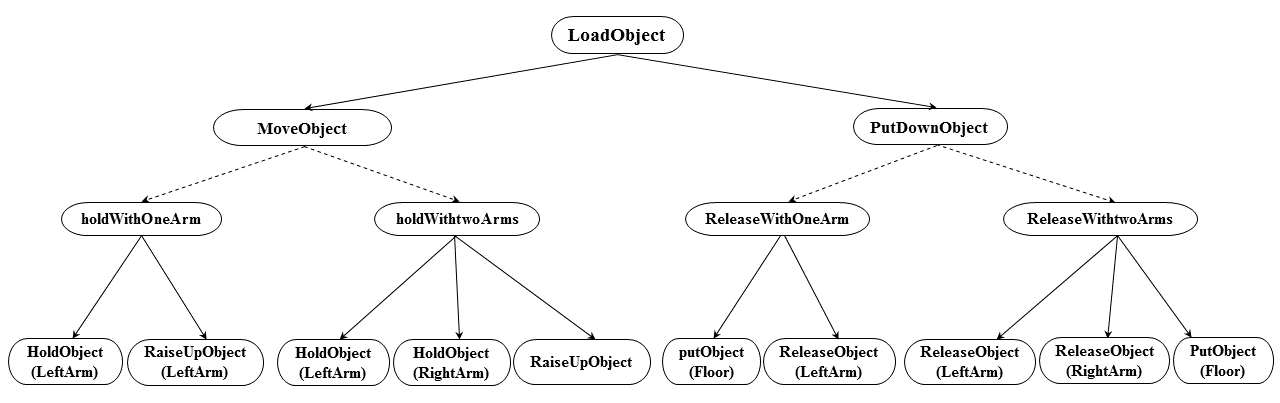
\includegraphics[width=\textwidth]{Figures/example1}
		 		\caption{Load Object task decomposition for robot arm motion}
		 	\end{figure*}
	
	\par In order to better understand our model, we present in this section an example of 	a robot responsible for charging object into trucks. The  goal task decomposition to achieve the load task is described in figure 1.
	 
	\par To load an object into the truck, the robot has to move it from its initial place and put it into the truck. The agent starts by decomposing the goal task "LoadObject", then the first task to perform is the "MoveObject" task. This task is defined with two recipes to hold the object. Depending on the object's  weight, the robot will choose the corresponding recipe as described in figure 1: the first recipe proposes the robot to use one arm if the object weight is below than 5 kilograms. The second recipe proposes to use both of the robot arms if the object weight is higher than 5 kilos and below than 10 kilos. The same is done for the "PutDownObject" task.
	\par If we consider an object with the weight of 20 kilos. The "LoadTask" execution is as performed as follows: The robot decomposes the "LoadObject" task. Next, it decomposes the "MoveObject" task. The robot tries the first recipe "holdWithOneArm".Thus it invokes a sensor to calculate the object's weight,the object is heavier than 5 kilos which doesn't correspond the the script of the applicability condition. Therefore, it tries the second recipe "holdWitwoArm" and holds the object with both of its arms but it fails again because the object is heavier than 10 kilos which make the applicability condition of the recipe also fails. At this moment, all the recipes to decompose the "MoveObject" task are inapplicable. by consequence, the execution is blocked with no possible task to execute. A breakdown is then reached by the robot. When a breakdown is detected, the robot has to think of a strategy or a plan to get out from this breakdown.  In the next section we present our proposition to overcome the breakdown problem. 
	
	
	
	\section{Hybrid model: Extending reactive HTNs with symbolic planning}
	
	%	In this section we present our proposition based on extending the reactive HTN with symbolic planner to recover from breakdowns.
%	\par Reactive HTNs don't look ahead to predict the future. Instead, they plan only for the next act to perform at every moment which make the agent reactive with the changes in its environment.  Nevertheless, as dynamic environment is unpredictable,  primitive task execution might lead to a dead end where no possible task can be performed next and a breakdown is detected. In order to recover from such breakdown, the agent has to think of a strategy, but reactive planning avoid long term prediction and without symbolic knowledge the agent has no way to think. 
	\par To overcome the breakdown problem, we propose in this paper, to extend the reactive HTN with a symbolic linear planner that construct a local strategy to recover from the faced breakdown. The hybrid system combines the reactive formalism of the HTN and the symbolic formalism of the linear planning system.
	To construct the symbolic knowledge requisite to the symbolic planner for reasoning. We propose thus,  to the HTN designer to extend all boolean procedures defined in the task's and recipe's conditions which the structure is similar to logical predicates  into a symbolic formalism. Since linear planner reason  on primitive tasks (i.e actions) (see section \ref{sec:symbolic}), the HTN designer extends only the primitive tasks which contains boolean procedures.
	\begin{algorithm}[h]
		\caption{ Reactive planning and plan recovery algorithm}
		\label{pseudoPSO}
		\begin{algorithmic}[]
			\Procedure{Hybrid system}{DomainKnowlege,Goal}
			\State $\pi \gets Reactive HTN \textit{(DomainKnowlege,Goal)}$
			\State \textbf{If} {($ \pi \gets\textit{Success} $)} 
			\State \Return $\textit{Success} $
			\State \textbf{else} $ plan \gets Recover(Goal)$
			\State If {(plan $=$ \textit{null})}
			\State \Return Failure
			\State \textbf{else} 
			\State {$ \textbf{foreach}$  action \textit{$a_i$} $\in$ plan }
			\State  $\textit{Discolog} (HTN,a_i) $
			
			
			\EndProcedure 
			\State
			\Procedure{Recover}{Goal}
			\State $\textit{Candidates}\gets\textit{findCandidate}{(G)} $
			\State \textbf{If} {$ \textit{Candidates = }\emptyset $} 
			\State \Return $\textit{null} $
			\State \textbf{else}  $\Pi \gets \emptyset$
			
			\State {$ \textbf{foreach} \textit{ candidate} \in \textit{Candidates}$}
			\State $\Pi += $ LinearPlanner(candidate, CurrentState)
			\State  $Cost \gets \{ cost(\pi) | \pi \in  \Pi \} $
			
			\State \Return $\pi \in \Pi$  with minimum cost$(\pi)$
			
			\EndProcedure
			\State
			\Procedure{FindCandidates}{Goal}
			\State {$ \textbf{foreach} \textit{ child} \in \textit{Goal}$}
			\State  {\textbf{If} (precondition(child)$!=\emptyset$ and \textit{status} (child)$\notin\{Done, Live, Blocked\})$}
			\State add precondition(child) to Candidates
			
			\State{\textbf{else If} (postcondition(child)$!=\emptyset$ and \textit{ status} (child)$ \in \{Failed\}$}
			\State add postcondition(child) to Candidates	
			\State  {\textbf{If} (\textit{status} $\in \{Live\}$ and nonPrimitive(child) and applicability(child)!=  $\emptyset)$}
			\State add App-condition(child) to Candidates
			
			\State $\textit{findCandidates} (children(child))$
			
			\State\Return Candidates
			
			\EndProcedure 
			%					\Procedure{FindCandidates}{Goal}
			%					\For{$ \textbf{each} \textit{ child} \in \textit{Goal}$}
			%					
			%					\If {$ \textbf{ status}$ (child) = failed}
			%					\State   add condition(child) to Candidates
			%					\EndIf
			%				
			%					\State $\textit{findCandidates} (children(child))$
			%					\EndFor
			%					\State \Return Candidates
			%	
			%					\EndProcedure 
		\end{algorithmic}
	\end{algorithm}
	\par The hybrid planning system proceeds as described in the algorithm  \ref{pseudoPSO}. It calls the reactive HTN  to achieve the goal. The environment is monitored at each step of the execution to check the success of the execution. Nevertheless, a breakdown might occur and make the  HTN execution fails. 
	\par When a breakdown is detected, the hybrid system invokes the recover algorithm. First, The recover algorithm traverses the hierarchy of the goal task to detect all the children tasks affected by the breakdown and attempt to propose a plan repair for them. A task is considered as failed if one of its conditions are no longer valid. Thus, the algorithm computes the task's failed conditions to repair them, using for that the task's status. A task status can be \textit{Live} (Task preconditions are valid and the task can be performed), \textit{ Done} (The task has been executed successfully),  \textit{Failed} (Task execution failed) or \textit{Blocked}  (Task preconditions are not valid). The algorithm then takes a task preconditions as candidate if its status is  \textit{Blocked}, or its postconditions if its status is \textit{Failed}. If the task is a compound task with its status to \textit{Live} and none of its recipes are valid then the applicability condition of those recipes are considered as candidates. For instance, taking back the example described in  section \ref{sec:example}, a breakdown is detected because no recipe can be applied to decompose the "MoveObject" task. The system, then calls the recover procedure to detect all the affected tasks by this breakdown. The candidates list includes both applicability conditions of the failed recipes, the postconditions of the "MoveObject" task and the "LoadObject" task.
	Note that a condition is considered as candidate only if it can be converted to a symbolic formalism. Otherwise, the recover procedure ignores this condition. 	
	\par Once the list of candidates has been determined, the linear planning system is called for each candidate. As linear planning systems plan to reach a state rather than achieving goals, then each task's conditions candidate is considered as goal state to reach.  The linear planner plans  for each candidate and tries to return a list of possible plans to recover from the breakdown. The most promising plan is calculated to be executed. We define the most promising plan as the shortest plan (i.e the plan that contains the less actions) to ensure local task repair and prevent other breakdowns due to the execution of pre-constructed plan. Thus, in the example, the planner proposes to repair the failed recipe "HoldWithTwoArm". Thus, the proposing plan repair consists on using a, existing task "Separate the Object" to separate the object into two objects of 10 kilos and load them separately.
	
	\section{Implementation and experimental results}
	\subsection{Discolog implementation}
	
	\par The proposition presented in this paper has been implemented using a reactive HTN called  Disco \cite{rich2009building} and a simple linear STRIPS planner, the STRIPS version used in this system is an existing  Prolog implementation proposed in \cite{poole1998computational}. Thus, we named the produced system \emph{Discolog}. 
	\par  Disco uses the ANSI/CEA-2018 standard for the procedural definition of its domain knowledge and a Java-based reactive planning system. Tasks are modeled using the XML format. Primitive tasks contain grounding script parameter defined	as JavaScript programs which represent the effect of  primitive task execution in the environment. 
	\par  The integration of STRIPS in the Disco system is performed using  \emph{tuProlog} \footnote{http://apice.unibo.it/xwiki/bin/view/Tuprolog/} framework. The use of  \emph{tuProlog} presents two mains advantages. First, \emph{tuProlog} is a Java-based framework that exploits a Prolog engine directly from a Java program. Thus, STRIPS can locally raised without any call to an external system. Second, it has specific libraries for the prolog predicates that eases the conversion of recovery candidates from the procedural knowledge to symbolic knowledge. 
	\subsection{Experiments and results}
	\par  In this section, we present ou experiment with the \emph{Discolog} system. The aim of this  experiment is first to validate the hybrid architecture of Discolog system. Second, we want to test the contribution of the symbolic knowledge in the performances of recovery. We make the assumption that the effectiveness of the recovery process is relied to the level of knowledge in the symbolic domain knowledge. In fact, we assume that the more information STRIPS planner gets from the procedural domain knowledge, the more effective recover plans it can generates. The result of this experiment should proves that plan recovery follows a monotonic evolution in function of the level of knowledge defined in STRIPS.

	\par In order to validate  Discolog, we had to test it on different HTNs domain knowledge and analyze its ability of recovery on every possible breakdown. Nevertheless, in the absence of accurate models including reactive and symbolic knowledge, we  implemented our own evaluation data. 
	\par As theses primary tests purpose is to validate the hybrid architecture of Discolog, we actually don't need a domain knowledge with a semantic description of its tasks. Therefore, we defined a procedural domain knowledge based only on synthetic data  structured in such way to ensure a believable execution.  Each compound task (T) is defined with a set of recipes (R) and each recipe is constituted by a set of children tasks (C) to decompose the parent task (T). Preconditions of compound task are propagated to its first child in each recipe, and the postconditions are propagated to its last child. 
	The rest of task children in each recipe are defined with chained conditions: The postconditions of the $task_i$ activate the preconditions of the $task_{i+1}$. Symbolic knowledge is extracted from the procedural one. Depending on the level of knowledge we want to study, we randomly extract primitive tasks from the HTN procedural knowledge.   The goal is to study the affect of the level of symbolic knowledge defined on recovery.
	\par We tested Discolog on different HTNs model. We denote ($\alpha$, $\beta$, $\gamma$)  respectively the depth of the HTN, number of recipes per each task, number task children per recipe. For each HTN, we varied first, the level of symbolic knowledge to be extracted \{25\%, 50\%, 75\%\} \footnote{0 \% of symblic knowledge means no possible recovery and 100 \% is not realistic taking in account the dynamic definition of environment}. For each level of knowledge, we randomly extracted different symbolic domain knowledge.  Second, the initial state is randomly defined. This later affects the decomposition that the HTN will choose and the plan recover procedure. 
	Once theses parameters are set, for each primitive task, a breakdown is caused and the plan recovery for this task is analyzed. The experiments have been done on two different HTN configuration as presented in table \ref{table}.
		\begin{table}[h]
				
				\centering % used for centering table
				\caption{Configuration of the HTNs } % title of Table
				\begin{tabular}{|c|c|c|c|} 
					\hline
					Configuration & Total Nb of nodes & Init state & Nb of symbolic DN\\
					\hline
					(3,3,3) & 91 & 10 & 60  \\
					(5,1,4) & 341 & 10 & 60  \\
					\hline
				\end{tabular}
				\label{table} % is used to refer this table in the text
			\end{table}
			
			
			\begin{figure}[t]
				\centering
				\begin{subfigure}[b]{0.5 \columnwidth}            
					\frame{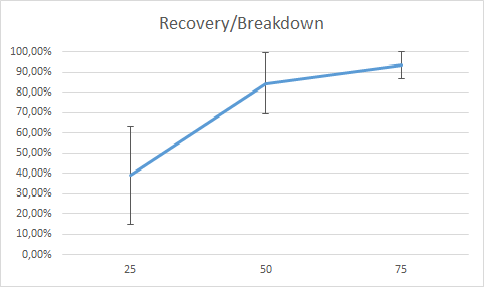
\includegraphics[width=6cm]{Figures/3.png}}
					\caption{ Recover rate for each level of knowledge}
					\label{Fig:Data3}
				\end{subfigure}
				%
				\hspace{1cm}
				%
				\begin{subfigure}[b]{0.5 \columnwidth}
					\centering
					\frame{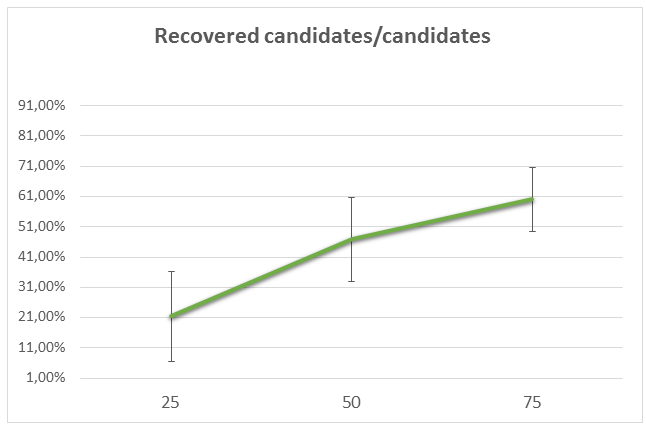
\includegraphics[width=6cm]{Figures/4.png}}
					\caption{Average number of candidates repaired for each level of knowledge}
					\label{Fig:Data4}
				\end{subfigure}
				\caption{Results for the (3, 3, 3) HTN}\label{fig:TOF}
			\end{figure}
			
			\begin{figure}[t]
				\centering
				\begin{subfigure}[b]{0.5 \columnwidth}            
					\frame{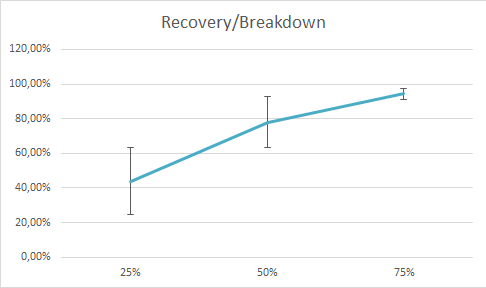
\includegraphics[width=6cm]{Figures/1.png}}
					\caption{ Recover rate for each level of knowledge}
					\label{Fig:Data1}
				\end{subfigure}
				%
				\hspace{1cm}
				%
				\begin{subfigure}[b]{0.5 \columnwidth}
					\centering
					\frame{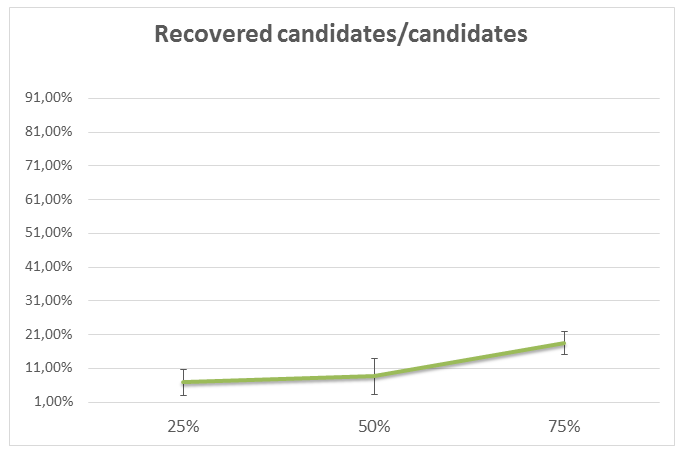
\includegraphics[width=6cm]{Figures/2.png}}
					\caption{Average number of candidates repaired for each level of knowledge}
					\label{Fig:Data2}
				\end{subfigure}
				\caption{Results for the (4, 1, 5) HTN}\label{fig:TOF2}
			\end{figure}	
	\par  Figures \ref{Fig:Data3} and  \ref{Fig:Data1} display the recover rate for HTNs. We notice that the hybrid system is able to propose plans recovery and switch between the procedural and the symbolic environment. Moreover, the results confirm our assumption: the graph follows a monotonic assumption in function of the symbolic knowledge. Thus, the more symbolic knowledge Discolog has the more it can recover from breakdowns. 

	The error bars defined in the graphs represent the standard deviations for each execution in function of the level of symbolic knowledge.  We notice that the less symbolic knowledge Discolog has the bigger is the standard deviation.  For the same HTN, Discolog gets different rates of performances. For example for HTNs defined with the 25 \% of symbolic knowledge, Discolog performances varies from  0\% to 65\%  of recover. This is noticed in the case of HTN with 25 \% and 50 \% of defined symbolic knowledge. Thus, HTNs  defined with limited symbolic domain knowledge, are unable to cover from all the possible breakdowns because of their lack of symbolic knowledge. 
	
	\par  Figures \ref{Fig:Data4} and \ref{Fig:Data2} show the average of the number of candidates repaired during the execution. The results for repairing  candidates also confirm our assumption. However, the error bars as demonstrated in graphs show that Discolog performances varies for repairing all the possible candidates and this independently of the level of symbolic knowledge defined. Theses result raise a new question of the quality of the symbolic knowledge defined by the designer. Symbolic knowledge is limited, then it has to be expressive and very representative of the agent policy, or Discolog will not have the precise knowledge to recover from all the possible breakdowns. 
	\par These tests are very promising but remain far from being definite experimental analysis. An extensive tests on a set of realistic domain knowledge is the object of futures works to detail the problematic of the quality of knowledge and test Discolog on real planning problems. 
	\section{Conclusion}
	\par In this paper we have presented \emph{Discolog}, an algorithm to recover from breakdowns in reactive HTN planning systems.  Despite the ability of reactive planning  to deal with high dynamic world,  breakdowns might occur because of the lack of knowledge on the different possible changes in the world and the ineptitude  of reactive HTN to reason in long term to define a recover strategy. 
	\par The proposed algorithm extends reactive HTNs with linear symbolic planner to produces a plan to recover from the breakdown. The symbolic knowledge is extracted from the procedural knowledge by the HTN designer. Thus if a breakdown is detected, the algorithm calculates the candidates (conditions which are not valid in the non-executed HTN tasks), then 
	STRIPS is called to propose plans to repair these conditions. The most promising plan is then converted to procedural formalism and executed. 
	\par The solution have been implemented. It combines a reactive HTN Disco with the symbolic linear planning system STRIPS in Prolog.  The
	results of our preliminary experiments  demonstrated, first, the ability of the hybrid planning system Discolog to propose viable plans recovery and for the different breakdowns. Second, the  contribution of symbolic knowledge in the performances of the recovery. Finally, the experiments raise another problematic of the quality of  knowledge in limited domain knowledge that we wish address. In addition, we intend to validate Discolog on real  applications such as social dialog systems, we believe that with real applications, we can study the problem of the quality of the symbolic knowledge.  
	\par Future prospects of this research are, first, to construct a modeling tool for HTN	model design. This tool will help the HTN designer in one hand to define the level of knowledge to integrate in the HTN. In the other hand, the system will use the history of breakdowns to propose adding knowledge in the HTN where breakdowns occurred. As second step, we propose to integrate Discolog in social dialog system between an agent and a human in order to support the dynamic nature of a social dialog.
	
	
	% if have a single appendix:
	%\appendix[Proof of the Zonklar Equations]
	% or
	%\appendix  % for no appendix heading
	% do not use \section anymore after \appendix, only \section*
	% is possibly needed
	
	% use appendices with more than one appendix
	% then use \section to start each appendix
	% you must declare a \section before using any
	% \subsection or using \label (\appendices by itself
	% starts a section numbered zero.)
	%
	
	
	%	\appendices
	%	\section{Proof of the First Zonklar Equation}
	%	\
	%	
	%	% use section* for acknowledgement
	%	\section*{Acknowledgment}
	%	
	
	
	
	
	% Can use something like this to put references on a page
	% by themselves when using endfloat and the captionsoff option.
	\ifCLASSOPTIONcaptionsoff
	\newpage
	\fi
	
	
	
	% trigger a \newpage just before the given reference
	% number - used to balance the columns on the last page
	% adjust value as needed - may need to be readjusted if
	% the document is modified later
	%\IEEEtriggeratref{8}
	% The "triggered" command can be changed if desired:
	%\IEEEtriggercmd{\enlargethispage{-5in}}
	
	% references section
	
	% can use a bibliography generated by BibTeX as a .bbl file
	% BibTeX documentation can be easily obtained at:
	% http://www.ctan.org/tex-archive/biblio/bibtex/contrib/doc/
	% The IEEEtran BibTeX style support page is at:
	% http://www.michaelshell.org/tex/ieeetran/bibtex/
	%\bibliographystyle{IEEEtran}
	% argument is your BibTeX string definitions and bibliography database(s)
	%\bibliography{IEEEabrv,../bib/paper}
	%
	% <OR> manually copy in the resultant .bbl file
	% set second argument of \begin to the number of references
	% (used to reserve space for the reference number labels box)
	\label{Bibliography}
	\bibliography{Bibliography} % The references (bibliography) information are stored in the file named "Bibliography.bib"
	\bibliographystyle{alpha}
	
	% biography section
	% 
	% If you have an EPS/PDF photo (graphicx package needed) extra braces are
	% needed around the contents of the optional argument to biography to prevent
	% the LaTeX parser from getting confused when it sees the complicated
	% \includegraphics command within an optional argument. (You could create
	% your own custom macro containing the \includegraphics command to make things
	% simpler here.)
	%\begin{biography}[{\includegraphics[width=1in,height=1.25in,clip,keepaspectratio]{mshell}}]{Michael Shell}
	% or if you just want to reserve a space for a photo:
	
	\begin{IEEEbiography}[{\includegraphics[width=1in,height=1.25in,clip,keepaspectratio]{picture}}]{John Doe}
		\
	\end{IEEEbiography}
	
	% You can push biographies down or up by placing
	% a \vfill before or after them. The appropriate
	% use of \vfill depends on what kind of text is
	% on the last page and whether or not the columns
	% are being equalized.
	
	%\vfill
	
	% Can be used to pull up biographies so that the bottom of the last one
	% is flush with the other column.
	%\enlargethispage{-5in}
	
	
	
	
	% that's all folks
\end{document}

